% $Header:
% /home/vedranm/bitbucket/beamer/solutions/conference-talks/conference-ornate-20min.en.tex,v
% 90e850259b8b 2007/01/28 20:48:30 tantau $

\documentclass{beamer}

% This file is a solution template for:

% - Talk at a conference/colloquium.
% - Talk length is about 20min.
% - Style is ornate.



% Copyright 2004 by Till Tantau <tantau@users.sourceforge.net>.
%
% In principle, this file can be redistributed and/or modified under
% the terms of the GNU Public License, version 2.
%
% However, this file is supposed to be a template to be modified
% for your own needs. For this reason, if you use this file as a
% template and not specifically distribute it as part of a another
% package/program, I grant the extra permission to freely copy and
% modify this file as you see fit and even to delete this copyright
% notice. 


\mode<presentation>
{
  \usetheme{Warsaw}
  % or ...

  \setbeamercovered{transparent}
  % or whatever (possibly just delete it)
}

\usepackage[italian]{babel}
% or whatever

\usepackage[latin1]{inputenc}
% or whatever

\usepackage{times}
\usepackage[T1]{fontenc}
% Or whatever. Note that the encoding and the font should match. If T1
% does not look nice, try deleting the line with the fontenc.
% \lstset{
%   language=XML,
%   basicstyle=\footnotesize,%\ttfamily,
%   columns=fullflexible,
%   morekeywords={encoding,
%     xs:schema,xs:element,xs:complexType,xs:sequence,xs:attribute}
% }

\title[Analisi di reti metaboliche] {Analisi di reti metaboliche
  basata su propriet\`a di connessione}

% \subtitle
% {Include Only If Paper Has a Subtitle}

\author[Massimo Nocentini] % (optional, use only with lots of authors)
{Massimo~Nocentini\\\texttt{massimo.nocentini@gmail.com}}
% - Give the names in the same order as the appear in the paper.
% - Use the \inst{?} command only if the authors have different
%   affiliation.

 \institute[UniversitaStudiFirenze] % (optional, but mostly needed)
 { Universit\`a degli Studi di Firenze }
%   \inst{1}%
%   Department of Computer Science\\
%   University of Somewhere
%   \and
%   \inst{2}%
%   Department of Theoretical Philosophy\\
%   University of Elsewhere}
% - Use the \inst command only if there are several affiliations.
% - Keep it simple, no one is interested in your street address.

\date[Tesi20120222] % (optional, should be abbreviation of conference name)
{Firenze, \today}
% - Either use conference name or its abbreviation.
% - Not really informative to the audience, more for people (including
%   yourself) who are reading the slides online

\subject{Theoretical Computer Science}
% This is only inserted into the PDF information catalog. Can be left
% out. 



% If you have a file called "university-logo-filename.xxx", where xxx
% is a graphic format that can be processed by latex or pdflatex,
% resp., then you can add a logo as follows:

\pgfdeclareimage[height=1.5cm]{university-logo}{logo/unifi}
\logo{\pgfuseimage{university-logo}}

% Delete this, if you do not want the table of contents to pop up at
% the beginning of each subsection:
\AtBeginSubsection[]
{
  \begin{frame}<beamer>{Contenuti}
    \tableofcontents[currentsection,currentsubsection]
  \end{frame}
}


% If you wish to uncover everything in a step-wise fashion, uncomment
% the following command: 

%\beamerdefaultoverlayspecification{<+->}


\begin{document}

\begin{frame}[plain]
  \titlepage
  % \begin{center}
  %   
\includegraphics[scale=.065]{logo/unifi}
  % \end{center}
\end{frame}

\begin{frame}{Contenuti}
  \tableofcontents[pausesections]
  % You might wish to add the option [pausesections]
\end{frame}


% Structuring a talk is a difficult task and the following structure
% may not be suitable. Here are some rules that apply for this
% solution: 

% - Exactly two or three sections (other than the summary).
% - At *most* three subsections per section.
% - Talk about 30s to 2min per frame. So there should be between about
%   15 and 30 frames, all told.

% - A conference audience is likely to know very little of what you
%   are going to talk about. So *simplify*!
% - In a 20min talk, getting the main ideas across is hard
%   enough. Leave out details, even if it means being less precise than
%   you think necessary.
% - If you omit details that are vital to the proof/implementation,
%   just say so once. Everybody will be happy with that.

\section{Motivazioni}

\subsection{Analisi di reti metaboliche}

\begin{frame}{Definizione di rete metabolica}
  % - A title should summarize the slide in an understandable fashion
  %   for anyone how does not follow everything on the slide itself.
  \begin{definition}
    Una rete metabolica \`e un insieme di reazioni chimiche che si
    verificano all'interno di una cellula.
  \end{definition}
  \`E interessante studiarle per:
  \begin{itemize}
  \item capire le propriet\`a fisiologiche e biochimiche delle
    cellule;
  \item ricostruire le reazioni che avvengono all'interno di
    organismi, sia batteri che esseri umani;
  \item studiare il comportamento della cellula in relazione al
    contesto che la ospita.
  \end{itemize}
\end{frame}

\begin{frame}{Codifica delle reti}{usando il linguaggio \emph{SBML}}
  \textbf{SBML} (\textbf{S}ystems \textbf{B}iology \textbf{M}arkup
  \textbf{L}anguage) \`e un linguaggio orientato alla descrizione di
  sistemi in cui entit\`a biologiche sono oggetto di manipolazioni
  eseguite da processi fisici.
  \begin{figure}
    
\includegraphics[scale=.6]{images/sbml-code-chunk.eps}
    \caption{Estratto della codifica del batterio Bartonella}
  \end{figure}
\end{frame}

\subsection{Lavori esistenti}

\begin{frame}{Ricerca dei \emph{Seed Compounds}}
  In \cite{Borenstein-Kupiec} si studiano le reti metaboliche per
  identificare i \emph{seed compounds}, ``interfacce'' tra la rete
  metabolica e il contesto che la ospita.

  Prima si identificano le interazioni della rete con il suo contesto
  (Figura A) poi, decomponendo la rete in componenti connesse, si
  scelgono i metaboliti di componenti sorgenti (Figura B) come
  \emph{seed compounds}.

  \begin{figure}
    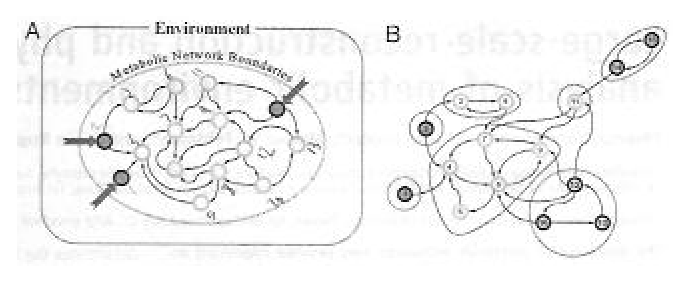
\includegraphics[scale=.6]{images/biology-scc-decomposition.eps}
  \end{figure}

\end{frame}

\begin{frame}{``Raccontare Storie''}
In \cite{Crescenzi-Marino} si studiano le reti metaboliche per
``raccontare'' tutte le \emph{storie} che vi sono contenute.
\begin{definition}
  Dato un grafo orientato $G = (\mathbb{B} \cup \mathbb{W}, E)$, una
  \emph{storia} \`e un sotto grafo aciclico $G' = (\mathbb{B} \cup
  \mathbb{W'}, E')$ di $G$ tale che $E' \subseteq E $ e:
  \begin{displaymath}
    \mathbb{W'} = \{w \in \mathbb{W}: indeg(w) > 0 \wedge outdeg(w)
    > 0\}
  \end{displaymath}
\end{definition}
L'insieme $\mathbb{B}$ \`e composto dai vertici a cui \`e permesso di
essere sorgenti o pozzi nelle \emph{storie} e ne identifica il loro
``ruolo''.
\end{frame}

\section{Nostro contributo}

\subsection{Obiettivi}

\begin{frame}{Analizzare reti, costruire $\mathbb{B}$ e verificare il
    metodo}
Gli obiettivi del nostro lavoro sono:
\begin{itemize}
\item<1-> rappresentare una rete mediante un grafo\\
  \footnotesize{astraendo dai molti dettagli di \emph{SBML}};
\item<2-> fornire strumenti per analizzare insiemi di reti\\
  \footnotesize{per avere informazioni sui metaboliti che appaiono in
    pi\`u di una rete};
\item<3-> costruire in modo automatico l'insieme $\mathbb{B}$\\
  \footnotesize{sfruttando le informazioni di tutte le reti studiate};
\item<4-> verificare se il metodo \`e accettabile\\
  \footnotesize{per misurare la validit\`a di $\mathbb{B}$}.
\end{itemize}
\end{frame}

\subsection{Metodologia}

\begin{frame}{Rappresentare una rete mediante un grafo}{Data una
    reazione \emph{non reversibile} $r$ tale che $reagenti(r) = \{ r_{1},
    \ldots, r_{n} \}$ e $prodotti(r) = \{ p_{1}, \ldots, p_{m} \}$}

  Costruiamo la relazione: $reagenti(r) \times prodotti(r)$.
  
    \begin{example}
      Con $reagenti(r) = \{ a, b, c, d \}$ e $prodotti(r) = \{a, e,
      f\}$ otteniamo il grafo:
      \begin{figure}
        \centering
        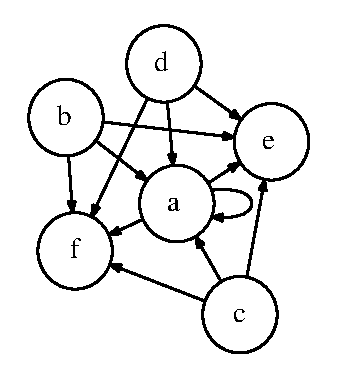
\includegraphics[scale=.6]{images/non-reversible-reaction-example.dot.eps}
        \label{fig:non-reversible-reaction-mapping}
      \end{figure}
    \end{example}
\end{frame}

\begin{frame}{Rappresentare una rete mediante un grafo}{Data una
    reazione \emph{reversibile} $r$ tale che $reagenti(r) = \{ r_{1},
    \ldots, r_{n} \}$ e $prodotti(r) = \{ p_{1}, \ldots, p_{m} \}$}

  Costruiamo la relazione: $(reagenti(r) \times prodotti(r)) \cup
  (prodotti(r) \times reagenti(r))$.
  
    \begin{example}
      Con $reagenti(r) = \{ a, b, c, d \}$ e $prodotti(r) = \{a, e,
      f\}$ otteniamo il grafo:
      \begin{figure}
        \centering
        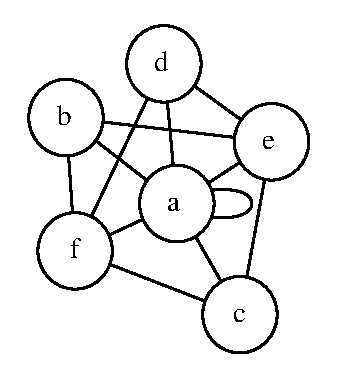
\includegraphics[scale=.6]{images/reversible-reaction-example.dot.eps}
        \label{fig:reversible-reaction-mapping}
      \end{figure}
    \end{example}
\end{frame}

\begin{frame}{Ricerca delle componenti fortemente connesse}
  Attualmente l'insieme $\mathbb{B}$ viene costruito in base a
  osservazioni e studi \emph{empirici}, costituito da metaboliti con
  propriet\`a particolari.

  Per costruirlo in modo automatico partizioniamo la rete in
  componenti connesse in quanto:
\begin{itemize}
\item<2-> \`e difficile assegnare il ruolo ad ogni vertice studiando
  l'intera rete date le sue dimensioni;
\item<3-> \`e possibile astrarre dai cicli ed identificare classi di
  metaboliti equivalenti;
\item<4-> due metaboliti equivalenti si producono a vicenda, pertanto
  gli associamo il ruolo della componente che li contiene;
\item<5-> se una componente \`e \emph{sorgente} o \emph{pozzo} nel
  ``meta grafo'' allora aggiungiamo i vertici che la compongono in
  $\mathbb{B}$.
\end{itemize}
\end{frame}

\subsection{Risultati}

\begin{frame}{Struttura delle reti}
  \begin{center}
    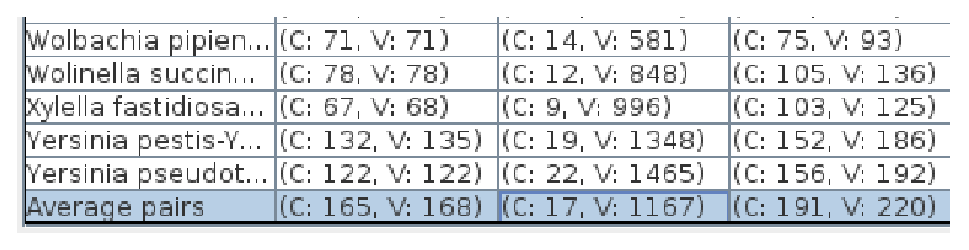
\includegraphics[scale=.5]{images/ResultViewer-table-with-average-row-selected-particular.eps}
  \end{center}
Tutte le reti hanno una struttura a ``clessidra'':
\begin{itemize}
\item molte componenti \emph{sorgenti} contenenti pochi vertici;
\item poche componenti \emph{intermedie} contenenti molti vertici;
\item molte componenti \emph{pozzo} contenenti pochi vertici.
\end{itemize}
\pause
\begin{alertblock}{Troppi vertici sorgente}
  Questo non \`e un buon risultato in quanto gli studi attuali mirano
  a reti con pochi vertici in $\mathbb{B}$.
\end{alertblock}
\end{frame}

\begin{frame}{Vertici con pi\`u ruoli in reti diverse}
  \begin{center}
    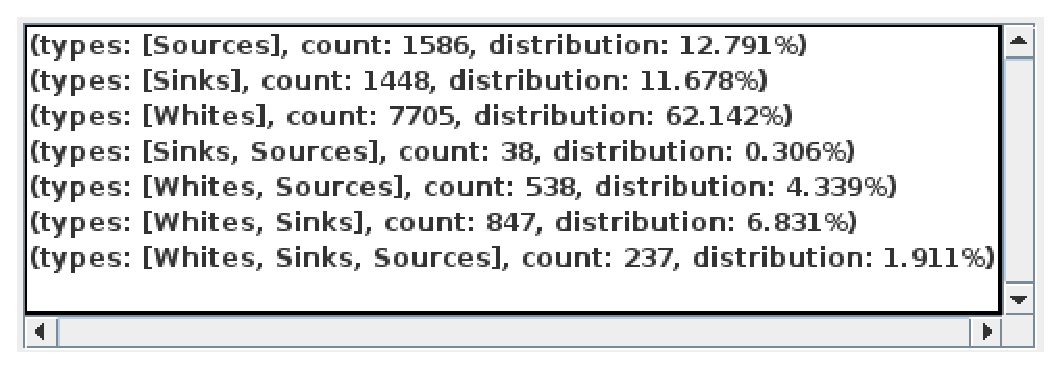
\includegraphics[scale=.5]{images/ResultViewer-grouping-table-zoom}
  \end{center}
  Studiando un insieme di reti, pi\`u del 10\% dei vertici non hanno
  un ruolo univoco.
  \pause
  \begin{alertblock}{Incertezza sulla costruzione di $\mathbb{B}$}
    Vertici con pi\`u di un ruolo inducono incertezza sul decidere la
    loro appartenenza all'insieme $\mathbb{B}$.
  \end{alertblock}
\end{frame}

\begin{frame}{Raffinare $\mathbb{B}$ rispetto ad un insieme di reti}
    \begin{center}
      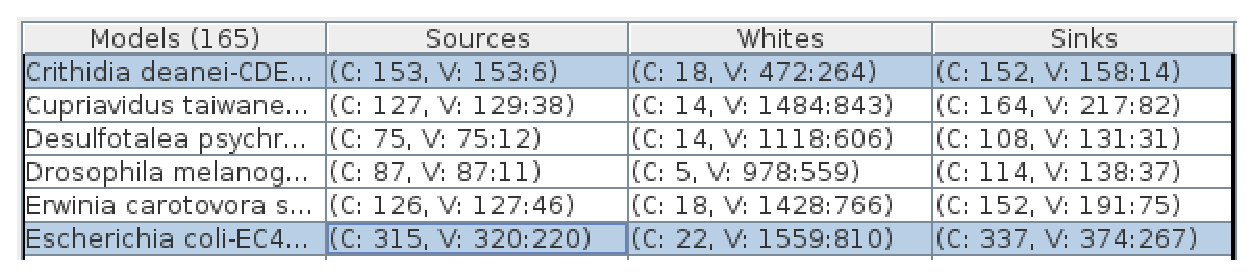
\includegraphics[scale=.3]{images/many-models-with-b-refinement}
  \end{center}
  Se consideriamo tutti i vertici che hanno un ruolo univoco rispetto
  ad un insieme di reti, \`e possibile raffinare ogni $\mathbb{B}$
  escludendo i vertici che non hanno un ruolo conforme.
\end{frame}


\section*{Sommario}

\begin{frame}{Riepilogo}
  % Keep the summary *very short*.
    \begin{itemize}
    \item costruire l'insieme $\mathbb{B}$ in modo automatico
      attraverso le componenti connesse \emph{non} produce risultati
      soddisfacenti;
    \item l'unico caso utile riguarda l'analisi di modelli singoli,
      anche se rimane il problema di avere molti vertici in
      $\mathbb{B}$.
    \end{itemize}
\end{frame}

% All of the following is optional and typically not needed. 
\appendix
\section<presentation>*{\appendixname}
\subsection<presentation>*{Riferimenti Bibliografici}

\begin{frame}%[allowframebreaks]
  \frametitle<presentation>{Riferimenti Bibliografici}
    
  \begin{thebibliography}{10}
    
  \beamertemplatearticlebibitems

  \bibitem{Crescenzi-Marino}
    P.~Crescenzi, A.~Marino et altri.
    \newblock {\em Telling Stories}.

  \bibitem{Borenstein-Kupiec}
    E.~Borenstein, M.~Kupiec, M.~Feldman, E.~Ruppin.
    \newblock {\em Large-scale reconstruction and phylogenetic analysis of
    metabolic environments}.

  \bibitem{Tarjan}
    R.~Tarjan.
    \newblock {\em Depth-First Search and linear graph algorithms}.

  \end{thebibliography}
\end{frame}

\end{document}

